\PassOptionsToPackage{subsection=false}{beamerouterthememiniframes}
\documentclass{beamer}

\usetheme{Szeged}
%\usepackage{pgfpages}
%\setbeameroption{show notes on second screen=right}
\setbeamertemplate{navigation symbols}{}
%\usecolortheme[named=black]{structure}
\definecolor{db}{HTML}{3A4454}
\definecolor{elblue}{HTML}{53687e}
\setbeamercolor{palette primary}{bg=blue,fg=white}
\setbeamercolor{palette secondary}{bg=blue,fg=white}
\setbeamercolor{palette tertiary}{bg=elblue,fg=white}
\setbeamercolor{palette quaternary}{bg=black,fg=white}
\setbeamercolor{structure}{fg=db} % itemize, enumerate, etc
\setbeamercolor{section in toc}{fg=black} % TOC sections
\setbeamercolor{frametitle}{bg=white,fg=elblue}
% Override palette coloring with secondary
\setbeamercolor{subsection in head/foot}{bg=gray,fg=white}

\setbeamertemplate{section in toc}{\inserttocsectionnumber.~\inserttocsection}

\usepackage{xurl}
\usepackage{amsmath,amsfonts}
\usepackage{tikz}
\usetikzlibrary{shapes.geometric, arrows}
\usefonttheme[onlymath]{serif}

\newcommand{\R}{\mathbb{R}}
\newcommand{\E}{\mathbb{E}}
\newcommand\dint{\mathord{\mathrm{d}}}
\newcommand{\M}{\mathbf{M}}
\newcommand{\A}{\mathbf{A}}
\newcommand{\B}{\mathbf{B}}

\begin{document}

\title{Charakteristische Funktionen}
%\subtitle{Am Beispiel von Git und GitHub}
\author{Maximilian Ernst}
\date{\today}
\begin{frame}
\titlepage
\end{frame}

\begin{frame}\frametitle{Inhalt}\tableofcontents\end{frame}

%%%%%%%%%%%%%%%%%%%%%%%%%%%%%%%%%%%%
\section{Motivation}
%%%%%%%%%%%%%%%%%%%%%%%%%%%%%%%%%%%%
\begin{frame}
\frametitle{Dualität}
Wir schauen auf zwei Seiten der selben Medaille.
\end{frame}

\begin{frame}
\frametitle{Beispiel 1}
Betrachte die Menge aller Kreise.

Die duale Menge ist die Menge alle einbeschriebenen Quadrate.
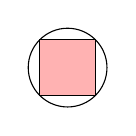
\begin{tikzpicture}
\node (start) [circle, minimum width=1cm, minimum height=1cm, text centered, draw=black] {};
\node (end) [rectangle, minimum width=0.7061cm, minimum height=0.7061cm, text centered, draw=black, fill=red!30] {};
\end{tikzpicture}

Die Relation $>$ für den Flächeninhalt bleibt erhalten. Wollen wir also wissen, ob ein Kreis größer als ein anderer ist, können wir stattdessen auch schauen, ob das einbeschrieben Quadrat größer ist.
\end{frame}

\begin{frame}
\frametitle{Beispiel 2}
Es gilt (bei fester Basis): jeder linearen Funktionen $f: \R^n \mapsto \R^n$ kann eineindeutig eine Matrix zugeordnet werden, die sogennante Darstellungsmatrix $\M_f$, sodass gilt:

$$f(x) = \M_fx$$

Die erhalten bleibende Struktur ist die Verknüpfung von Funktionen:

$$\M_{f \circ g} = \M_f \M_g$$

Außerdem gilt:

$$f \; \text{ist bijektiv} \iff \M_f \; \text{ist invertierbar}$$
\end{frame}

\begin{frame}
\frametitle{Ein einfacher Beweis}
$\A, \B \in \R^{n \times n}$ sind invertierbar $\implies \A \B$ ist invertierbar
\hfill \break
\hfill \break
Beweis:
\begin{enumerate}
  \item \textbf{Gehe in die duale Menge:} \hfill \break
  Es existieren lineare Funktionen $f, g: \R^n \to \R^n$ sodass
  \begin{itemize}
    \item[--] $\A$ die Darstellungsmatrix von $f$ ist
    \item[--] $\B$ die Darstellungsmatrix von $g$ ist
    \item[--] $f, g$ sind bijektiv
  \end{itemize}
  \item \textbf{Führe den Beweis in der dualen Struktur:} \hfill \break
  Da $f, g$ bijektiv sind, ist auch $f \circ g$ bijektiv.
  \item \textbf{Gehe zurück in die ursrüngliche Menge:} \hfill \break
    Es ist dann $\A \B$ die Darstellungsmatrix von $f \circ g$, und     da $f \circ g$ bijektiv ist, ist $\A \B$ invertierbar.
\end{enumerate}


\end{frame}

\begin{frame}
\frametitle{Ziel}
Jeder (reellwertigen) Zufallsvariable ein möglichst "einfaches" mathematisches "Objekt" zuordnen, sodass wir Dinge einfacher berechnen/beweisen können.
\end{frame}

\begin{frame}
\frametitle{Ziel}
\begin{itemize}
    \setlength\itemsep{1em}
    \item[--] Verteilung der Summe unabhängiger Zufallsvariablen
    \item[--] Berechnung von Momenten
    \item[--] Berechnung von Verteilungskonvergenzen
\end{itemize}
\end{frame}

\begin{frame}
\frametitle{Mittel}
Wir bestimmen eine (strukturerhaltende) bijektive Abbildung aus der Menge aller reellwertigen Zufallsvariablen in einen andere Menge.

Dann zeigen wir, dass wir anstelle mit den Zufallsvariablen zu rechnen, auch viel einfacher mit ihrem "Partner" rechnen können.
\end{frame}

\begin{frame}
\frametitle{Definition}
Für eine Zufallsvariable X mit Werten in $\R$ bezeichnet
\begin{align} \label{eq1}
\varphi^X(u) &= \E[e^{iuX}] \\
 & = \int_{\R} e^{iux} \dint P^X(x)\\
 & = \int_{\R} \cos(ux) \dint P^X(x) + i \int_{\R} \sin(ux) \dint P^X(x)
\end{align}

ihre charakteristische Funktion.

\end{frame}

\begin{frame}
\frametitle{Eigenschaften}
$\varphi$ sollte besonders "einfach" sein
\hfill \newline
\begin{itemize}
    \setlength\itemsep{1em}
    \item[--] $\varphi(0) = 1$
    \item[--] $|\varphi| \leq 1$
    \item[--] gleichmäßig stetig
\end{itemize}
\end{frame}

%%%%%%%%%%%%%%%%%%%%%%%%%%%%%%%%%%%%
\section*{Referenzen}
%%%%%%%%%%%%%%%%%%%%%%%%%%%%%%%%%%%%

\frame{
\frametitle{Links}

}
\end{document}
